%{
% \documentclass[12pt,ngerman]{/Users/dominik-cau/Documents/Lernen/Uni/Promotion/Vorlagen/Bayreuth/Exercise/AssignmentClass}
\documentclass[12pt,ngerman]{AssignmentClass}
% \documentclass{article}
%\documentclass[12pt, english]{AssignmentClass}


%----------------------------------------------------------------------------------------
%	PACKAGES AND OTHER DOCUMENT CONFIGURATIONS
%----------------------------------------------------------------------------------------
% Template-specific packages
\usepackage[utf8]{inputenc} % Required for inputting international characters
\usepackage[T1]{fontenc} % Output font encoding for international characters
\usepackage{mathpazo} % Use the Palatino font
\usepackage{wasysym} % for flash-symbol
\usepackage{graphicx} % Required for including images
\usepackage{amsmath}
\usepackage{listings} % Required for insertion of code
\usepackage{siunitx}
\usepackage{pnets}
\usepackage[most]{tcolorbox} % Grey Deadline Bar
\DeclareMathAlphabet{\mathpzc}{OT1}{pzc}{m}{it}
% Initialize comment sections
\usetheme{light-theme}
\excludecomment{dark-theme}
\excludecomment{solution}


%----------------------------------------------------------------------------------------
%	SET VERSION
%----------------------------------------------------------------------------------------
%\includecomment{dark-theme}
\includecomment{solution}


%----------------------------------------------------------------------------------------
%	ASSIGNMENT INFORMATION
%----------------------------------------------------------------------------------------
%\setlanguageEnglish
%\setlanguageGerman
% \begin{dark-theme}
% 	\usetheme{dark-theme}
% 	\excludecomment{light-theme}
% \end{dark-theme}
\title{Übung 2 Lösung} % Assignment title
\instructor{Yorck Zisgen}
\class{Generative Künstliche Intelligenz} % Course or class name
\term{Sommersemester 2024}
% \topics{Begriffe $\bullet$ Kontrollflussmuster $\bullet$ Organisationseinheiten}
\topics{28.05.2024}
%----------------------------------------------------------------------------------------
%}

\begin{document}
	\maketitle

    % Header Deadline Bar
    %{
    \noindent % Ensures the box spans the entire width
    \begin{tcolorbox}[colback=gray!20, % Background color as light gray
                      colframe=gray!20, % Frame color same as background
                      boxrule=0pt, % No border
                      sharp corners, % Sharp corners
                      valign=center, % Vertically centered text
                      halign=center, % Horizontally centered text
                      height=2cm] % Height of the box
    \LARGE \bfseries Beispiellösung % Bold text
    \end{tcolorbox}
    %}

    \section{Prompting Strategien 1}
        \begin{enumerate}[a)]
            \item Geben Sie ein Beispiel für \textbf{Zero-Shot} Prompting. Für welche Anwendungsfälle eignet sich diese Strategie?

            \textit{Beispiel:} 'Explain the concept of Generative Adversarial Networks in simple words.'
            
            \textit{Anwendungsfälle:} Üblicherweise einfache, kleine Aufgabenstellungen oder innerhalb von Chained Prompting.
            
            \item Geben Sie ein Beispiel für \textbf{One-Shot} Prompting. Was ist der Vorteil gegenüber dem Zero-Shot Prompting?

            \textit{Beispiel:} 'Can you provide the results of recent NBA games? Please structure the output as follows: 'Date: [MM/DD/YYYY], Team A vs. Team B, Final Score: [Team A Score]-[Team B Score], Top Performer: [Player Name], Points: [Player Points]'.'

            \textit{Vorteil:} Durch die Vorgabe einer Musterlösung entspricht die Antwort des LLMs deutlich eher den Erwartungen des Benutzers.
             
            \item Nutzen Sie \textbf{Few-Shot} Prompting, um einen Urlaub zu planen.

            You are an expert travel planner. Your task is to plan a detailed one-week vacation itinerary for different types of travelers. Below are a few examples of itineraries you have created. Use these examples as a guide to create a new itinerary for a family with two young children who want to visit Paris, France.\\

            \textbf{Example 1: Solo Traveler to Tokyo, Japan}\\
            Day 1: Arrival and Check-in.\\
            Arrive at Narita Airport. Check-in at a hotel in Shinjuku. Evening: Explore Shinjuku Gyoen National Garden.\\
            Day 2: Shibuya and Harajuku\\
            Morning: Visit the Meiji Shrine. Afternoon: Shopping and lunch in Harajuku. Evening: Shibuya Crossing and Hachiko Statue.\\
            Day 3: Cultural Experience\\
            Morning: Visit Senso-ji Temple in Asakusa. Afternoon: Sumida Aquarium and Tokyo Skytree. Evening: Traditional Japanese dinner in Asakusa.\\
            Day 4: Day Trip to Mount Fuji\\
            Full day: Bus tour to Mount Fuji and the surrounding areas.\\
            Day 5: Museums and Art\\
            Morning: Visit the Tokyo National Museum. Afternoon: TeamLab Borderless digital art museum. Evening: Dinner in Odaiba.\\
            Day 6: Technology and Anime\\
            Morning: Explore Akihabara, the electronics district. Afternoon: Visit the Gundam Base and the Pokémon Center. Evening: Experience a themed café.\\
            Day 7: Departure\\
            Morning: Last-minute shopping in Ginza. Afternoon: Check-out and travel to Narita Airport for departure.\\
            
            \textbf{Example 2: Couple's Getaway to Santorini, Greece}\\
            Day 1: Arrival and Check-in\\
            Arrive at Santorini Airport. Check-in at a cliffside hotel in Oia. Evening: Dinner with a view of the sunset over the caldera.\\
            Day 2: Beach Day\\
            Morning: Visit Red Beach. Afternoon: Relax at Perissa Beach. Evening: Seafood dinner by the beach.\\
            Day 3: Explore Fira\\
            Morning: Take a cable car ride in Fira. Afternoon: Visit the Archaeological Museum of Thera. Evening: Stroll through the shops and dine in Fira.\\
            Day 4: Wine and Dine\\
            Morning: Wine tasting at Santo Wines Winery. Afternoon: Visit a local vineyard. Evening: Dinner at a traditional Greek taverna.\\
            Day 5: Boat Tour\\
            Full day: Boat tour to the volcanic islands and hot springs. Evening: Sunset cruise with dinner on board.\\
            Day 6: Historical Sites\\
            Morning: Visit Akrotiri Archaeological Site. Afternoon: Explore Ancient Thera. Evening: Return to Oia for a sunset dinner.\\
            Day 7: Departure\\
            Morning: Relax and enjoy the hotel amenities. Afternoon: Check-out and travel to Santorini Airport for departure.\\

            \item Ihr Team soll um eine technische Mitarbeiterstelle erweitert werden. Verwenden Sie \textbf{Chained Prompting}, um die Bewerbung zu lesen und zu evaluieren. Listen Sie alle Prompts auf, mit denen Sie zu einer Einstellungs- oder Ablehnungsentscheidung gelangt sind.


            Zur Bearbeitung der Aufgabe habe ich mir eine Jobbeschreibung und eine Bewerbung generieren lassen (das ist nicht Teil der Aufgabenstellung, aber machte die Bearbeitung leichter):
            \begin{itemize}
                \item \textit{Generate a job description for a software developer that needs good skills in Python and React, basic frontend development skills, some years of experience in both, and SQL skills.}
                \item \textit{Now generate an application for this job by a software developer that has Python experience for 10 years, react experience for 3 years, no SQL knowledge, and considers his UI skills average.}
            \end{itemize}
            
            Die Chained Prompts zur Entscheidung, ob ein Bewerber angenommen werden sollte, könnten folgendermaßen aussehen:
            \begin{itemize}
                \item \textit{Read the job description and the application. Does the applicant possess any Python skills? If so, how many years of practical experience does he have?}
                \item \textit{Based on his Python skills, does the applicant also know how to create a frontend?}
                \item \textit{And can he also connect the frontend to our database?}
                \item \textit{Based on your prior findings, would you advise to sign the applicant, or would you rather reject him?}
            \end{itemize}	
            
        \end{enumerate}


    
    \section{Prompting Strategien 2}
        Erklären Sie den Unterschied zwischen \textit{Iterative Prompting} und \textit{Chained Prompting}.\\
        Wann würden Sie welche Strategie verwenden?\\

        \textbf{Iterative Prompting} verwendet denselben Prompt wiederholt, um ihn schrittweise (iterativ) so zu verbessern, dass in einem einzigen Schritt das gewünschte Ergebnis erzielt wird. Der resultierende Prompt ist dadurch mitunter oft komplex, lässt sich aber als Einheit leicht wiederverwenden.\\
        
        Bei \textbf{Chained Prompting} wird eine Reihe von Prompts hintereinander verarbeitet. Diese nutzen die Ergebnisse voriger Prompts (den Kontext), um eine Aufgabenstellung schrittweise zu lösen. Die entstehenden Prompts sind dadurch für sich sehr verständlich, die Wiederverwendbarkeit ist jedoch aufwendiger.

    
    \section{LLM-Techniken}
        Erklären sie die Aufgabe und die Funktionsweise der folgenden Techniken:
        \begin{enumerate}[a)]
            \item Chunking

            \textbf{Chunking} zerlegt eine Informationsquelle in kleinere Einheiten ("Chunks", auch "Splits" genannt), damit diese in das Kontextfenster eines Sprachmodells passt. Je nach verwendetem Chunker lassen sich Chunk-Größe und Overlap einstellen.
            
            \textit{Hinweis:} In der Literatur werden die Begriffe 'Chunk' und 'Split', 'Chunking' und 'Splitting' oder 'Chunker' und 'Splitter' jeweils teils synonym verwendet.
            
            \item Embedding

            \textbf{Embedding} wandelt einen Chunk oder einen Anfrage in einen Embedding-Vektor um. Ein Embedding-Vektor entspricht einer Reihe von Zahlen, auf welcher die Nähe zu anderen Chunks oder Anfragen gemessen werden kann. 
            
            \item Dense Retrieval

            \textbf{Dense Retrieval} setzt nicht wie Keyword Search auf eine größtmögliche Gleichheit von Begriffen in Anfrage und gespeicherten Chunks, sondern verwendet die jeweiligen Embedding-Vektoren, um auf ihnen eine größtmögliche Ähnlichkeit zu ermitteln. Aus der Anfrage und dem über den Embedding-Vektor ermittelten relevantesten Chunk aus der Vektordatenbank wird dann eine Antwort generiert.
        \end{enumerate}


    
    \section{LLM-Anwendung mittels LangChain}
        Sie möchten den Customer Support ihres Unternehmens durch den Einsatz eines ChatBots entlasten. Dieser wird auf der Unternehmenshomepage verfügbar sein und soll Kundenanfragen entgegennehmen und beantworten.
        Modellieren Sie eine mehrgliedrige LangChain, um mögliche Benutzereingaben zu verarbeiten. Sie sollten mindestens in der Lage sein, Anfragen zu Rechnungen, Anfragen zu Lieferungen und Beschwerden zu erkennen und entsprechend zu verarbeiten.\\

        \begin{figure}
            \centering
            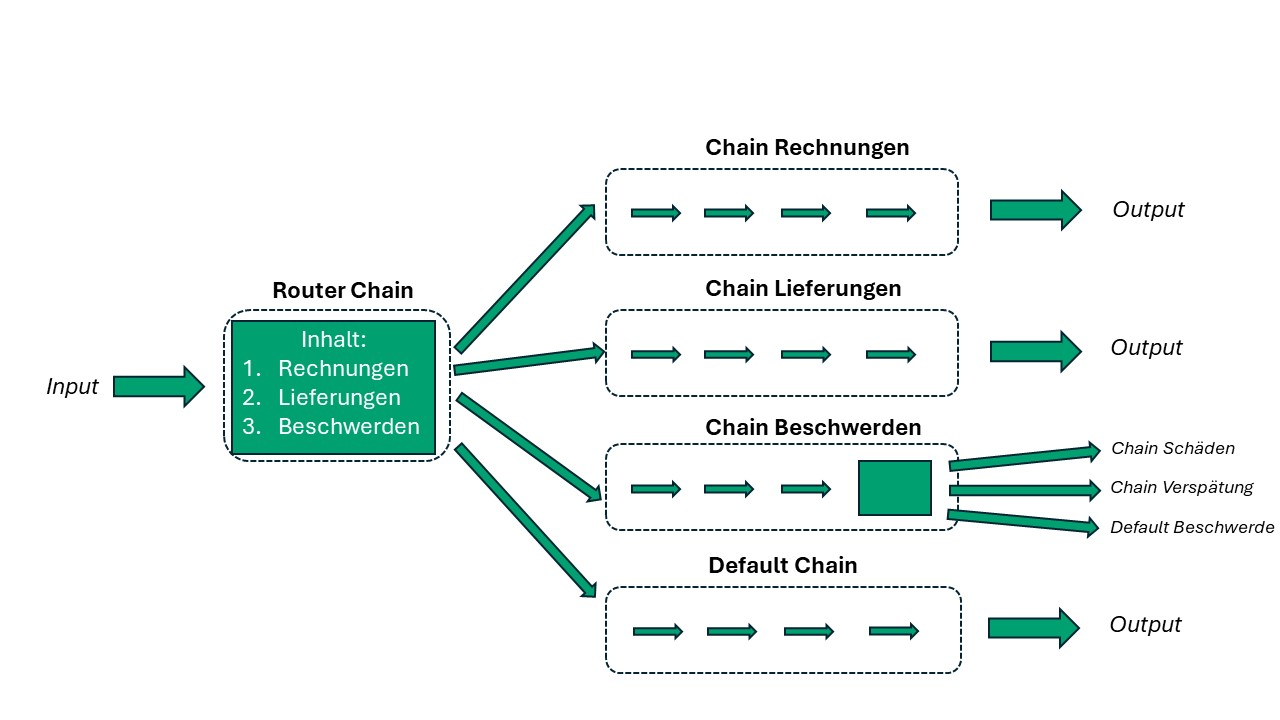
\includegraphics[width=1\linewidth]{Übung 2/Lösung/Aufgabe_4.jpg}
            \caption{LangChain für Customer Support}
            \label{fig:LangChain}
        \end{figure}

        Die modellierte LangChain in Abb. \ref{fig:LangChain}enthält eine Router Chain zur Analyse der Kundenanfrage und zur Weiterleitung an eine geeignete Chain. Sollte keine geeignete ermittelt werden, gibt es eine Default Chain. Diese könnte einen Prompt beinhalten, der gezielte Nachfragen stellt. Es sind spezielle Chains für die Themengebiete Rechnungen, Lieferungen und Beschwerden vorhanden. Diese beinhalten dann als SimpleSequentialChain oder als SimpleChain eine Vielzahl von LLMChains, um die Verarbeitungsschritte durchzuführen.\\

        In Erweiterung der Aufgabenstellung endet hier beispielsweise die Beschwerde-Chain in einer weiteren Router Chain, um den konkreten Grund der Beschwerde zu ermitteln und die Beschwerde an eine geeignete Chain zu delegieren. Auch hier gibt es wieder eine Default Chain für den Fall, dass der genaue Beschwerdegrund nicht ermittelt werden kann.

    
    \section{Reflexion und Diskussion}
        Reflektieren Sie Ihre bisherigen Erfahrungen im Umgang mit Generativer KI.
        \begin{enumerate}[a)]
            \item Welche Limitationen von ChatGPT sind Ihnen bisher bei der Verwendung aufgefallen?
            \item Wie wirken sich diese Limitationen auf Ihr Nutzungsverhalten aus?
        \end{enumerate}

        \noindent Diese Aufgabe geht auf Ihre individuellen bisherigen Erfahrungen mit Generativer KI ein. Eine Beispiellösung ist hierdurch nicht sehr sinnvoll.


\end{document}
